\section{Bond Graphs}
\begin{figure}[H]
    \centering
    \begin{minipage}{.5\textwidth}
        \centering
        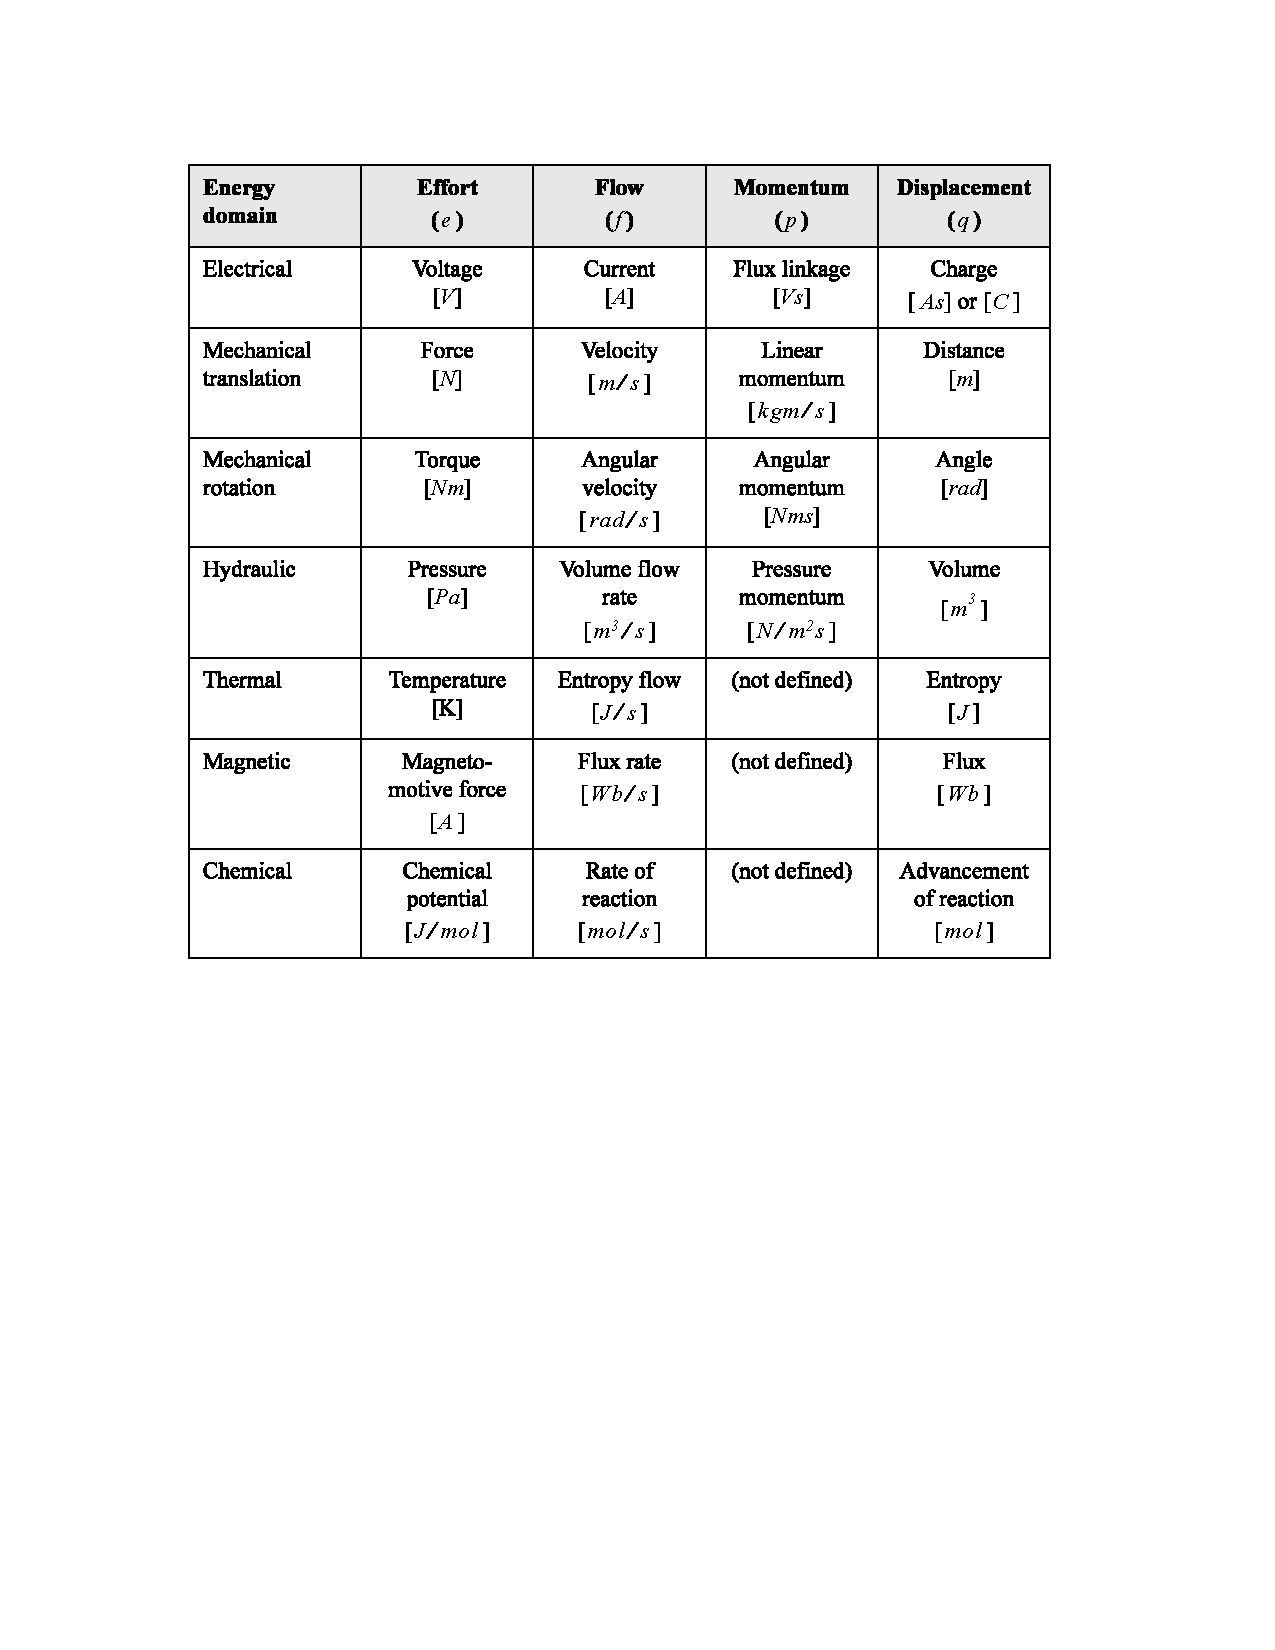
\includegraphics[width=.9\linewidth]{figures/Tabell_EnergyDomain.pdf}
        \label{fig:bond_graph1}
        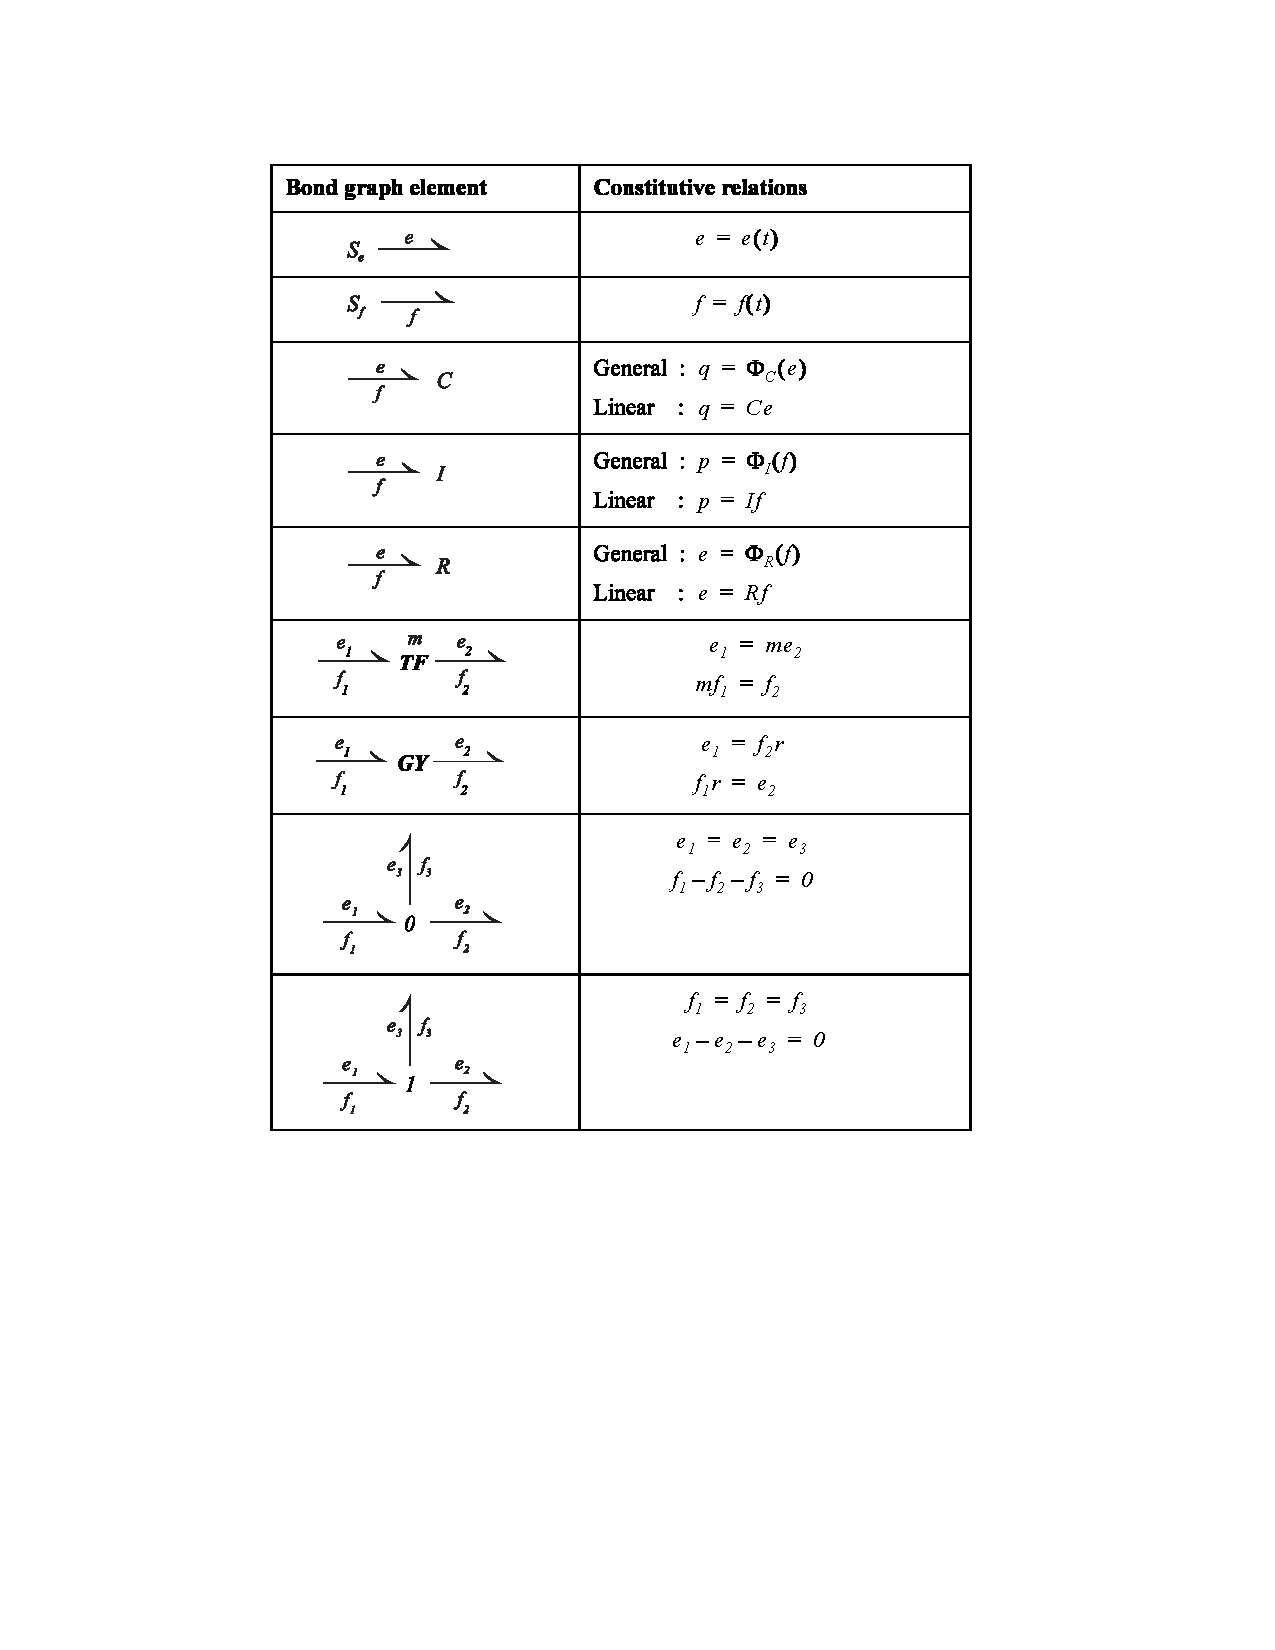
\includegraphics[width=.9\linewidth]{figures/Tabell_GraphElements.pdf}
        \label{fig:bond_graph2}
    \end{minipage}%
    \begin{minipage}{.5\textwidth}
        \centering
        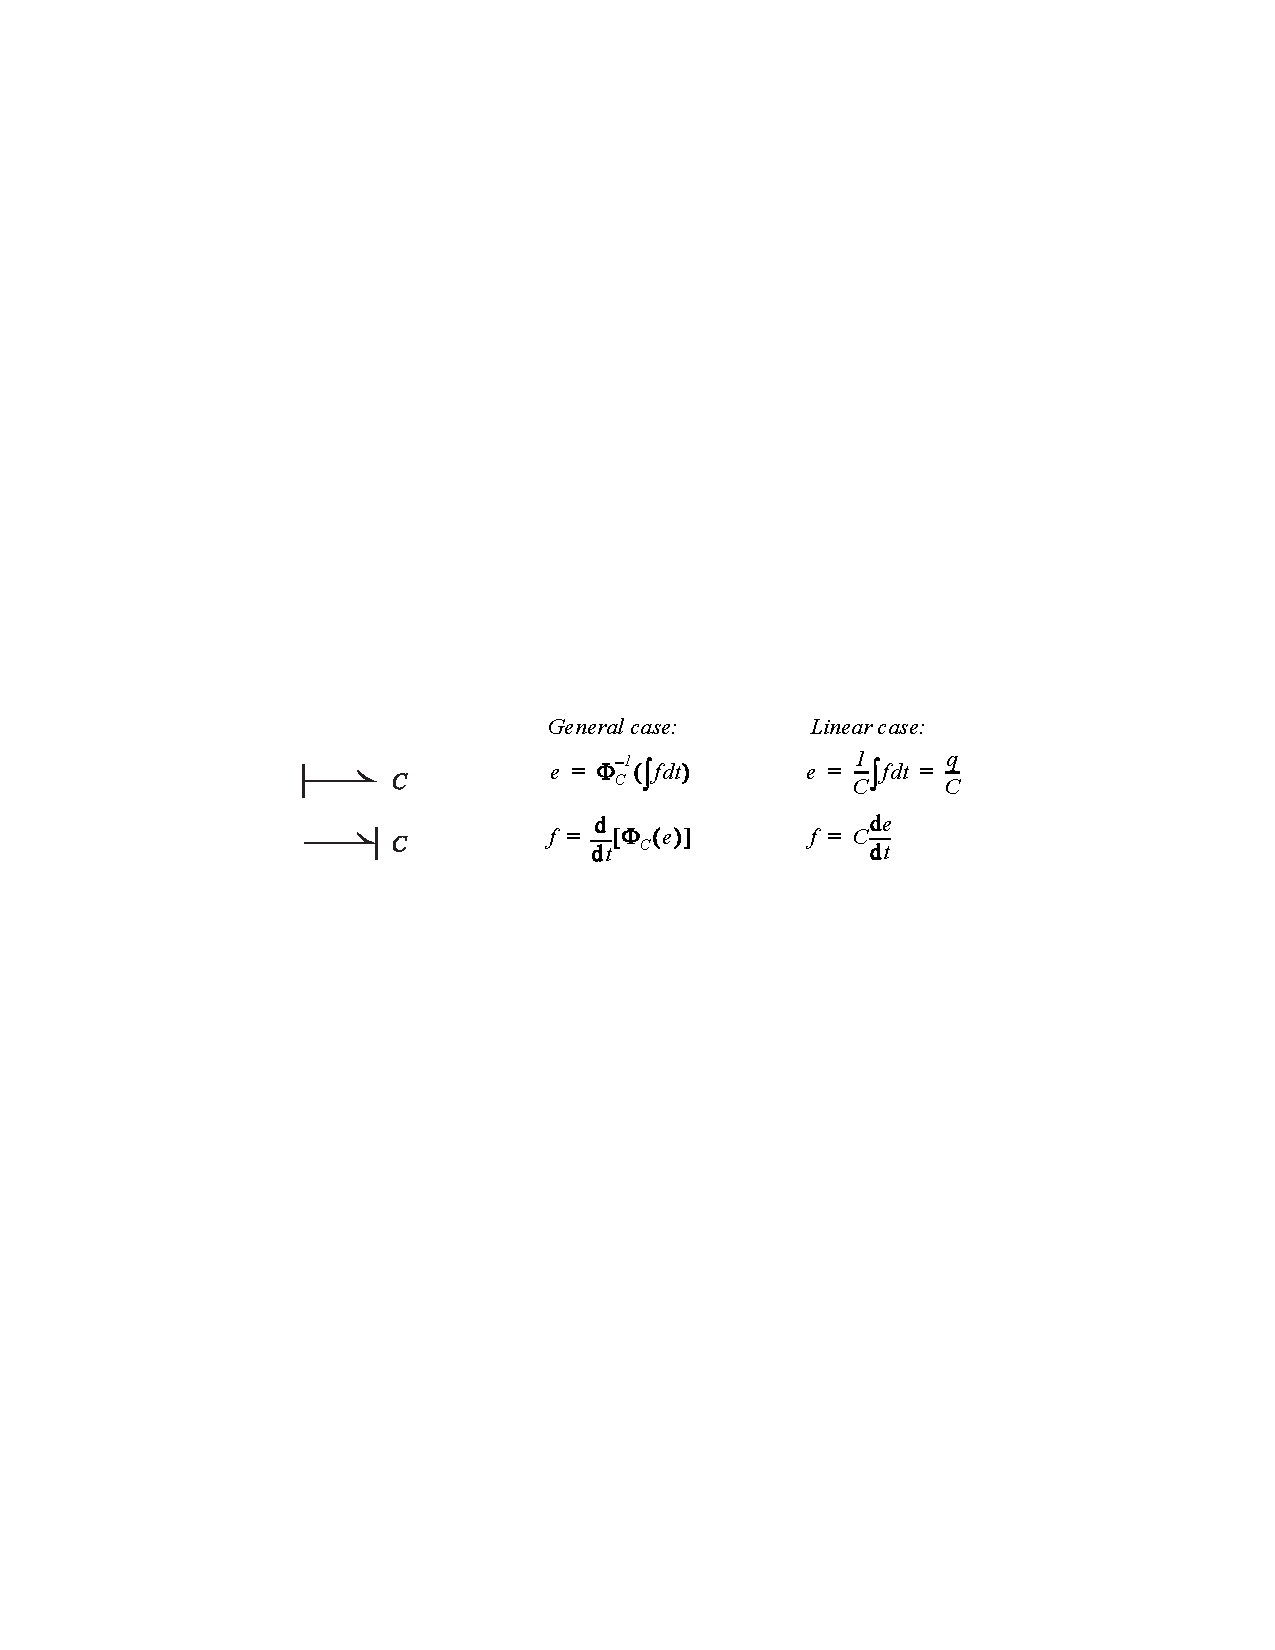
\includegraphics[width=.9\linewidth]{figures/fig45.pdf}
        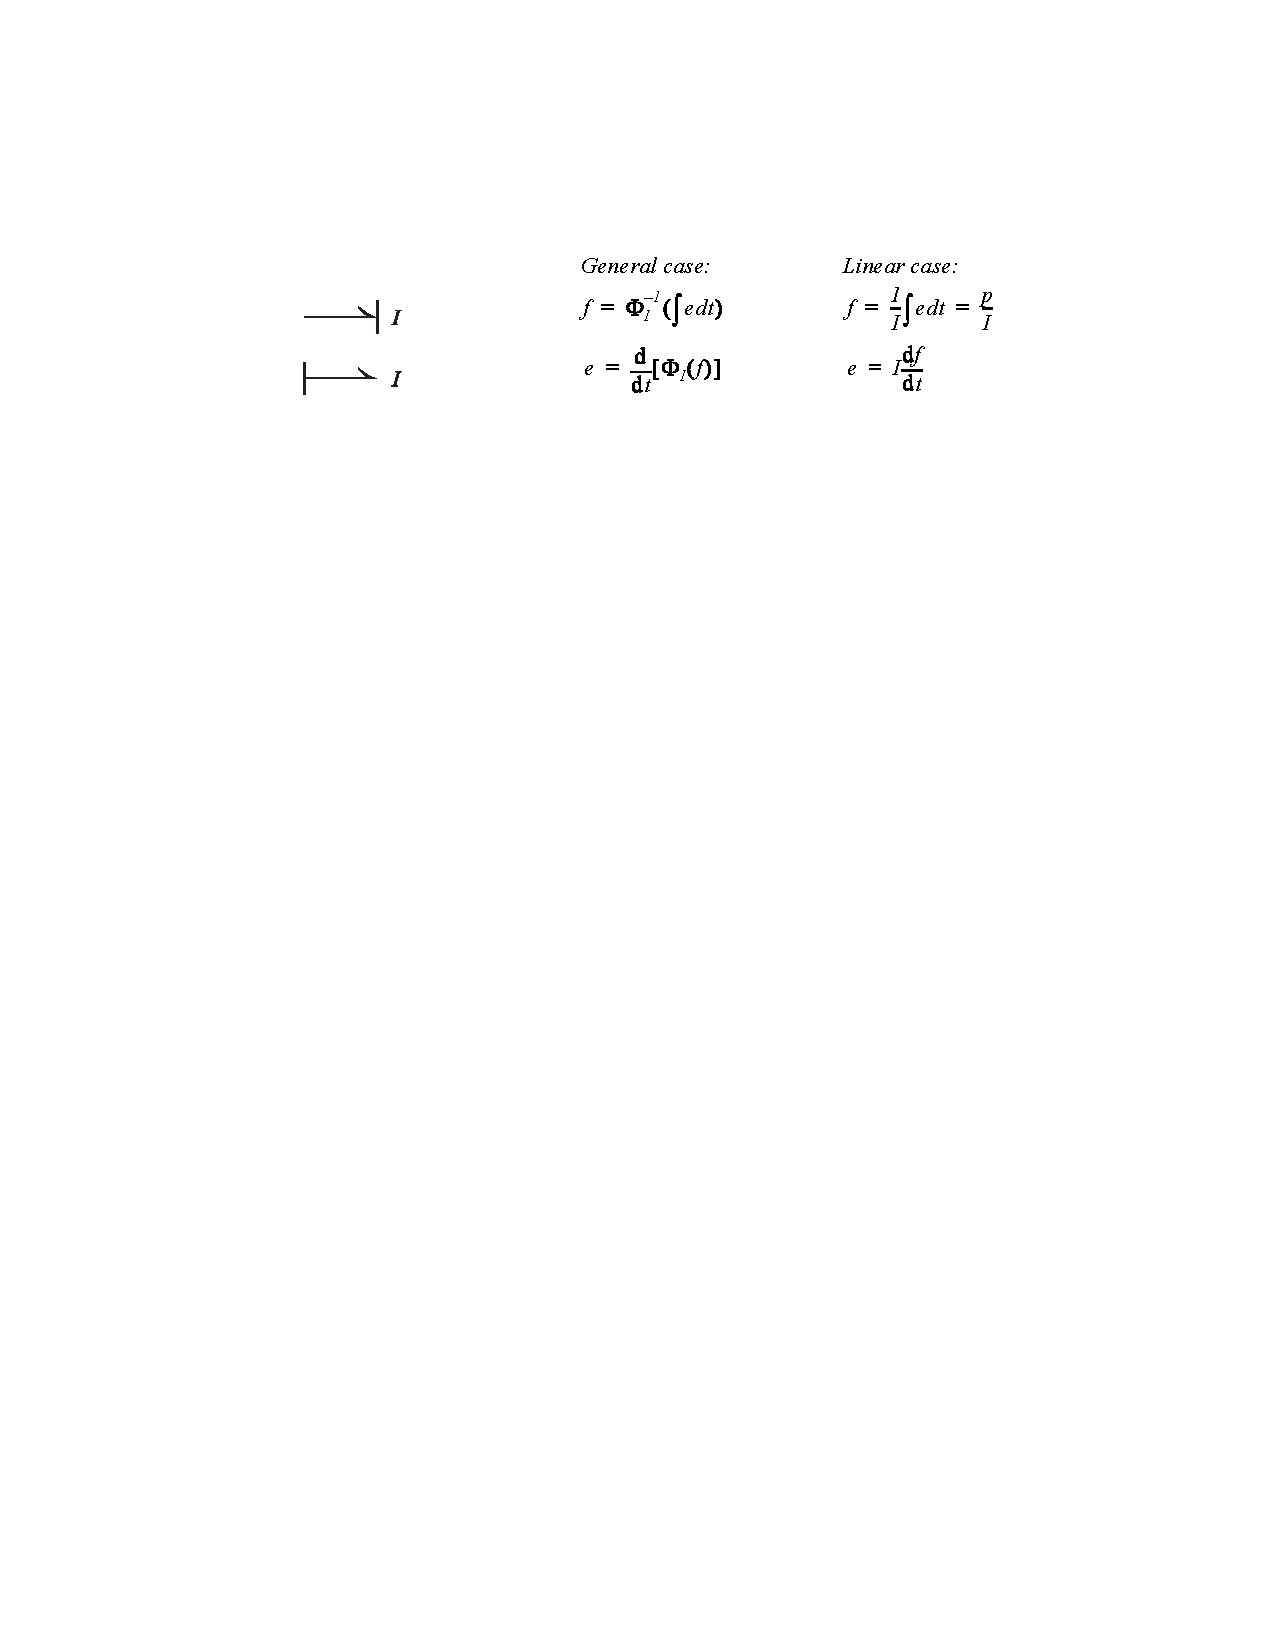
\includegraphics[width=.9\linewidth]{figures/fig46.pdf}
        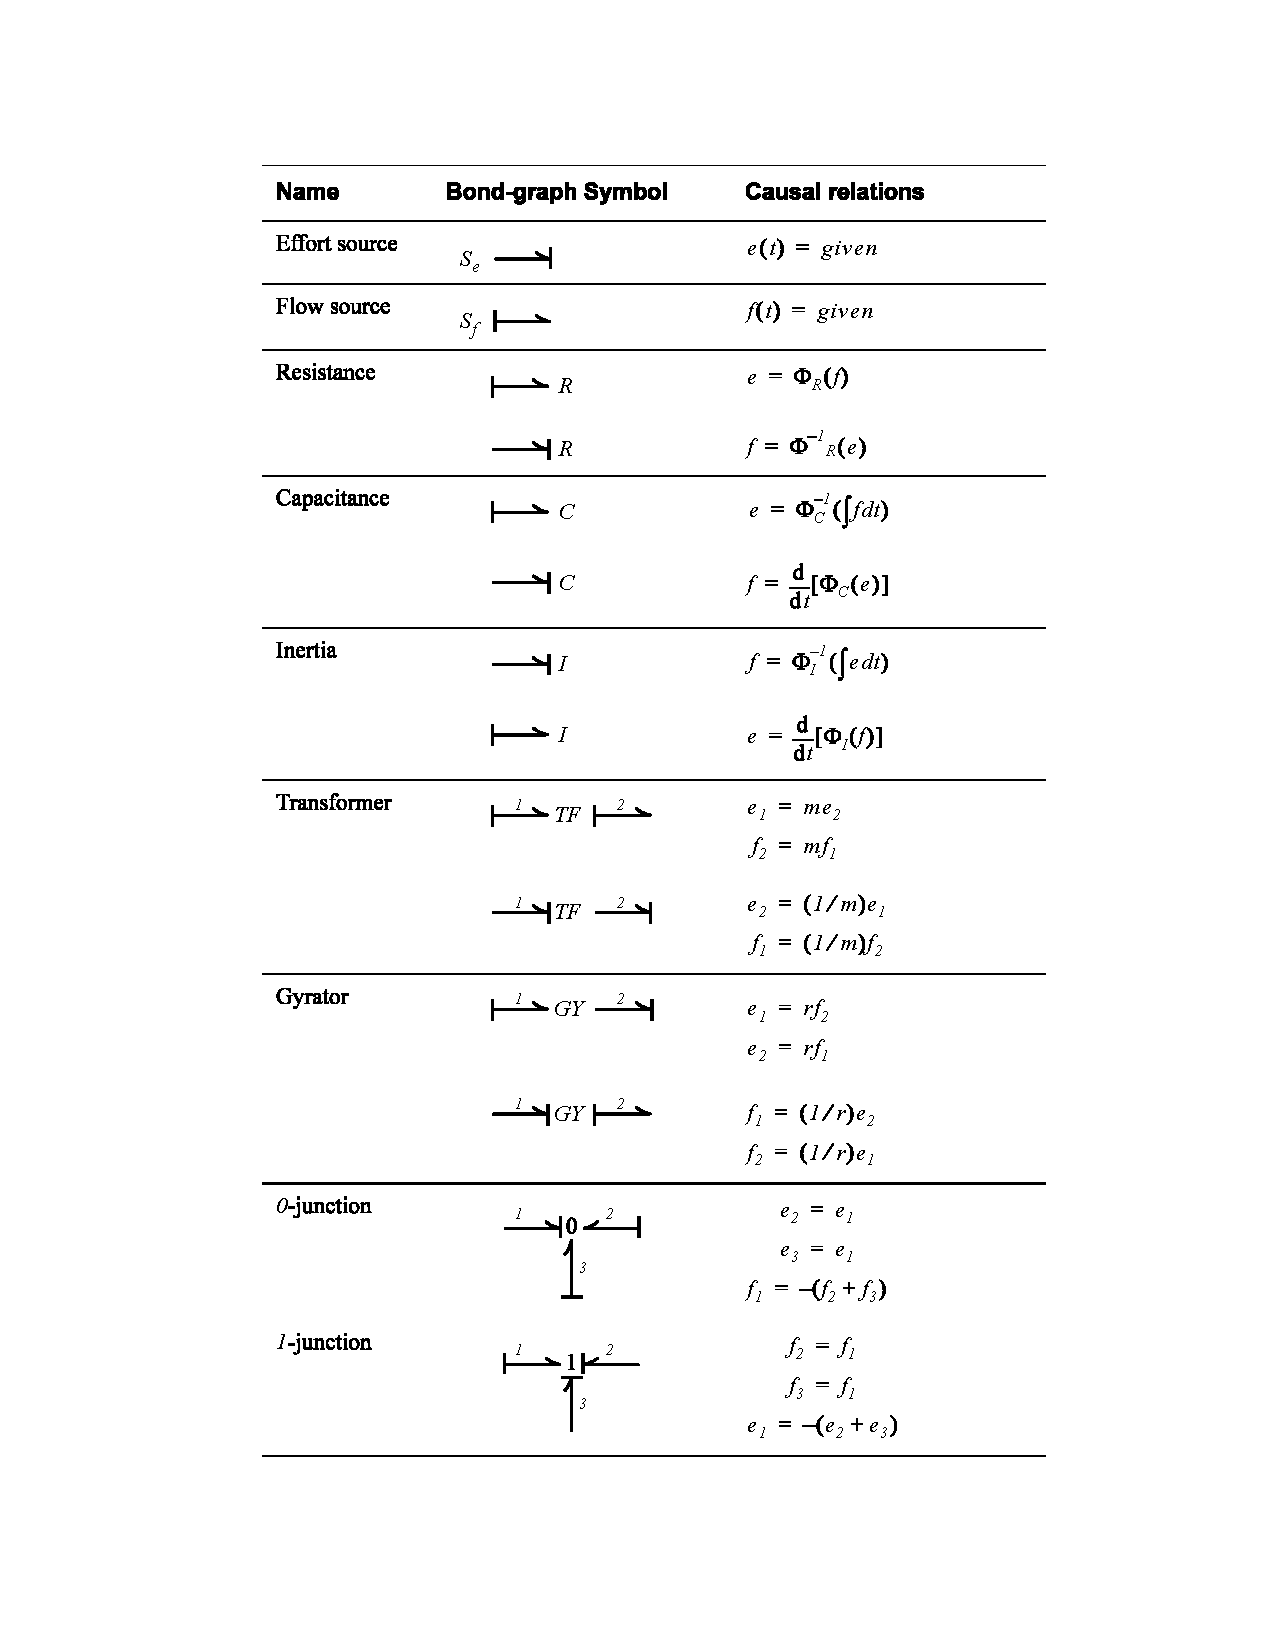
\includegraphics[width=.9\linewidth]{figures/Tabell_CausalRelations.pdf}
        \label{fig:bond_graph3}
        \fbox{\parbox{\linewidth}{
            \textbf{Generally:}\newline
            $p(t) = \int_{0}^{t} e(t)\,dt + p(0) \Rightarrow \dot{p} = e$\newline
            $q(t) = \int_{0}^{t} f(t)\,dt + q(0)  \Rightarrow \dot{q} = f$\newline
            $P(t) = e(t)f(t), \quad E(t) = \int_{0}^{t} P(t) \,dt = \int_{0}^{t} e(t)f(t) \,dt$
        }}
    \end{minipage}
\end{figure}
\textbf{Finding state-space model: }\newline
For all $I$ and $C$ elements with integral causality, set your states $\mathbf{x} = [p_i, p_j, q_k, q_l]$, where $i,j,k,l$ are the indices of the elements with integral causality. $I$ and $C$ elements with derivative causality are not part of your states!!